% !TEX root = main.tex
% Main text: abstract through conclusion. General-K statements, constants and proofs are in the appendix.
\begin{abstract}
A Transformer can contain an exact program for counting the letters of a prompt, both one that
writes only the final count and one that writes every running count. We ask which of these programs
gradient training actually finds, and prove three results for counting with $n$ hidden updates.
(1)~\emph{Outcome supervision is hard:} near small initialization, every Transformer term that reads
few letters gets gradient signal of order $\lambda^n$, where $\lambda<1$ is set by the letter
frequency, and outcome training stays on a plateau for time $\lambda^{-n}$.
(2)~\emph{Step supervision is easy:} displayed running counts keep a gradient signal that decays
only polynomially in $n$, joint gradient flow learns each transition in time $O(\varepsilon^{-4}\log\frac1\varepsilon)$, and step
training learns attention routing from zero position biases in polynomial time.
(3)~\emph{Same family, opposite outcomes:} in a model family that contains exact executors for both
formats, step gradient flow reaches positive margins on every transition from every seed in an explicit open set,
while outcome gradient flow from the same seeds converges to a suboptimal minimum with accuracy
$(1+\lambda^{n-1})/2$.
Experiments confirm the $\lambda^{-n}$ plateau and the trap, and show that step training learns routing jointly.
\end{abstract}

% ===================================================================
\section{Introduction}
\label{sec:intro}

Training on intermediate steps makes many reasoning tasks learnable
\citep{nye2021scratchpads,wei2022cot,lightman2023verify}. Is that because steps give more labels,
or because they change which program gradient descent can reach? We answer this for the simplest
task where the question is non-trivial: counting how often a query letter occurs, modulo two.

The task has one parameter that controls everything. Each letter is the query letter with
probability $p<1/2$; write $\lambda=1-2p$. An outcome label is the parity of all $n$ letters, so a
feature that reads only $k$ of them sees the label through $n-k$ letters it never observed, and each
unseen letter multiplies the correlation by $\lambda$ (\cref{fig:chain}). A step label is the next
running count, which depends on one new letter only.

\paragraph{Contributions.} We prove that this difference decides what training reaches.
\begin{itemize}[leftmargin=*,itemsep=2pt,topsep=2pt]
\item \textbf{Outcome is hard} (\cref{sec:outcome}). Near small initialization, a two-block Transformer
reads few letters at a time; the answer-dependent part of its outcome gradient is $O(\varepsilon\lambda^n)$ (\cref{thm:main}) and outcome
training stays near initialization for time $\lambda^{-n}$ (\cref{thm:outcome-end}).
\item \textbf{Step is easy} (\cref{sec:step}). The step gradient keeps a rule signal that decays
only polynomially in $n$ (\cref{thm:separation}); joint gradient flow learns every transition in time
$O(\varepsilon^{-4}\log\frac1\varepsilon)$ from aligned and misaligned seeds (\cref{thm:joint}), and step training learns where to attend
from zero position biases in polynomial time (\cref{thm:routing}).
\item \textbf{Same family, opposite outcomes} (\cref{sec:matched}). In a family containing exact
executors for both formats, the same seeds lead step flow to positive margins on every transition and outcome flow to
a suboptimal minimum (\cref{thm:matched}). The failure is a property of the outcome loss, not of
missing capacity.
\end{itemize}

\paragraph{Relation to \citet{kim2024parity}.} Kim and Suzuki prove that a Transformer learns parity with
teacher-forced chain of thought but not without it. Our setting differs in three ways. \emph{Task:} they
use worst-case $k$-parity, which is hard for any gradient method by a statistical-query argument;
counting with $p<1/2$ is a much easier target whose difficulty $\lambda$ can be tuned, so the fact that
outcome training still stalls points to the supervision format rather than the hardness of the task.
\emph{Architecture:} they use position-only attention, a fixed link function and one large gradient
step; we analyse a two-block Transformer for the plateau, and gradient flow that learns routing and
features jointly for the positive results. \emph{Kind of negative result:} theirs holds for every
algorithm with an approximate gradient oracle, which is stronger in form than our gradient-flow
plateau near small initialization. In exchange we obtain an explicit horizon dependence $\lambda^{-n}$,
and a same-family trap that rules out the explanation that outcome training merely lacks capacity.

% ===================================================================
\section{Setup}
\label{sec:setup}
\label{sec:setting}

\paragraph{Task.} A prompt has a start bit $s_0$, uniform on $\{0,1\}$, and letters $w_1,\ldots,w_n$ drawn
i.i.d.\ from an alphabet in which the query letter $w^\star$ has probability $p\in(0,1/2)$. With
$b_t=\mathbf 1[w_t=w^\star]$, the running count is
\[
 s_t=s_0+b_1+b_2+\cdots+b_t\pmod 2,\qquad t=1,\ldots,n .
\]
In sign form, put $S=(-1)^{s_0}$ and $C_t=(-1)^{b_t}$. Then
\begin{equation}
 (-1)^{s_n}=S\,C_1C_2\cdots C_n,\qquad \E[C_t]=1-2p=\lambda .
 \label{eq:tracking}
\end{equation}
So the answer is a product of signs, as in parity, but each sign is biased towards $+1$. The
\emph{contraction coefficient} $\lambda\in(0,1)$ is the only property of the task that enters our
bounds. For counting modulo $K$ the same role is played by the largest modulus of a nontrivial
Fourier coefficient of one letter (\cref{def:lambda}); \cref{app:contraction} proves every result of
\cref{sec:outcome,sec:step} for general $K$.

\begin{figure}[t]
\centering
\resizebox{\linewidth}{!}{% Conceptual figure: counting modulo K as a cyclic chain, and what each supervision format sees.
\begin{tikzpicture}[>=Stealth, font=\small,
  state/.style={circle, draw=royalazure!80!black, fill=royalazure!12, minimum size=7mm, inner sep=0pt},
  tok/.style={rectangle, rounded corners=2pt, draw=black!45, fill=black!4, minimum width=7mm, minimum height=5.5mm, inner sep=1pt},
  sup/.style={rectangle, rounded corners=2pt, draw=royalazure!80!black, fill=royalazure!12, minimum width=7mm, minimum height=5.5mm, inner sep=1pt},
  hid/.style={rectangle, rounded corners=2pt, draw=black!30, dashed, fill=white, text=black!45, minimum width=7mm, minimum height=5.5mm, inner sep=1pt}]

% ---------------- (a) cyclic chain ----------------
\begin{scope}[shift={(0,0)}]
  \foreach \i/\lab in {0/0, 1/1, 2/2, 3/{K{-}1}} {
    \node[state] (c\i) at ({90-\i*90}:1.25) {$\lab$};
  }
  \foreach \i/\dir in {0/90, 1/0, 2/-90, 3/180} {
    \draw[->, black!55] (c\i) to[out=\dir+28, in=\dir-28, looseness=6] node[pos=0.5, font=\scriptsize, fill=white, inner sep=0.5pt] {$1{-}p$} (c\i);
  }
  \draw[->, thick, royalazure] (c0) to[bend left=22] node[font=\scriptsize, above right=-1pt] {$p$} (c1);
  \draw[->, thick, royalazure] (c1) to[bend left=22] node[font=\scriptsize, below right=-1pt] {$p$} (c2);
  \draw[->, thick, royalazure, dashed] (c2) to[bend left=22] node[font=\scriptsize, below left=-1pt] {$p$} (c3);
  \draw[->, thick, royalazure] (c3) to[bend left=22] node[font=\scriptsize, above left=-1pt] {$p$} (c0);
  \node[align=center, font=\footnotesize] at (0,-2.6)
    {$s_t=s_{t-1}+b_t\ (\mathrm{mod}\ K)$\\[2pt] $\mathbf T=(1-p)\,\mathbf I+p\,\mathbf R$};
  \node[font=\small\bfseries] at (-2.3,1.75) {(a)};
\end{scope}

% ---------------- (b) what each format supervises ----------------
\begin{scope}[shift={(3.4,0.95)}]
  \node[font=\small\bfseries] at (-0.35,0.8) {(b)};
  % outcome row
  \node[anchor=west, font=\footnotesize] at (0,0.8) {Outcome: supervise $s_n$ only};
  \node[tok] (o0) at (0.45,0) {$s_0$};
  \node[tok] (ow1) at (1.35,0) {$w_1$};
  \node[hid] (os1) at (2.25,0) {$s_1$};
  \node[tok] (ow2) at (3.15,0) {$w_2$};
  \node[hid] (os2) at (4.05,0) {$s_2$};
  \node at (4.85,0) {$\cdots$};
  \node[tok] (own) at (5.65,0) {$w_n$};
  \node[sup] (osn) at (6.55,0) {$s_n$};
  \draw[decorate, decoration={brace, amplitude=4pt, mirror}, black!60] (1.0,-0.42) -- (6.0,-0.42)
    node[midway, below=4pt, font=\footnotesize, align=center] {$n$ hidden letters: each Fourier mode contracts by $\le\mixrate$ per letter};
  % step row
  \node[anchor=west, font=\footnotesize] at (0,-1.75) {Step: supervise every $s_t$ from the displayed $s_{t-1}$};
  \node[tok] (p0) at (0.45,-2.55) {$s_0$};
  \node[tok] (pw1) at (1.35,-2.55) {$w_1$};
  \node[sup] (ps1) at (2.25,-2.55) {$s_1$};
  \node[tok] (pw2) at (3.15,-2.55) {$w_2$};
  \node[sup] (ps2) at (4.05,-2.55) {$s_2$};
  \node at (4.85,-2.55) {$\cdots$};
  \node[tok] (pwn) at (5.65,-2.55) {$w_n$};
  \node[sup] (psn) at (6.55,-2.55) {$s_n$};
  \draw[rounded corners=3pt, thick, lightmauve!80!black] (1.83,-2.95) rectangle (3.55,-2.15);
  \draw[->, thick, lightmauve!80!black] (3.55,-2.55) -- (ps2.west);
  \node[font=\footnotesize, align=center] at (3.5,-3.45) {one local transition $(s_{t-1},w_t)\mapsto s_t$: innovation $\ge1-\mixrate^2$};
\end{scope}
\end{tikzpicture}
}
\caption{\textbf{One counting process, two views of it.}
(a)~Counting is a Markov chain: each letter keeps the count with probability $1-p$ and advances it with probability $p$.
(b)~Outcome supervision labels only $s_n$, so a feature that reads $k$ letters sees the label through
$n-k$ unseen steps, and its correlation shrinks like $\mixrate^{n-k}$ (\cref{thm:main}). Step supervision
displays the previous count and labels the next one, one step of the chain, which keeps a rule signal of variance $1-\mixrate^2$
(\cref{thm:separation}). The figure shows general $K$; the main text uses $K=2$.}
\label{fig:chain}
\end{figure}

\paragraph{Two formats.} Both formats see the same prompt. The \emph{outcome loss} $\Lout$ is the
cross-entropy of the final count $s_n$. The \emph{step loss} $\Lstep$ is the teacher-forced cross-entropy of
each transition: from a displayed count $s$ and the next letter $w$ to the next count $s'$, which is $s+1$ if $w=w^\star$
and $s$ otherwise (mod $2$), averaged over the positions $t\ge2$.

\paragraph{Model.} We use a Transformer with two causal attention/ReLU blocks, relative position
biases, no LayerNorm and a linear readout; $\bm\theta$ denotes all parameters.

\begin{proposition}[Both programs exist]
\label{prop:represent}
With widths linear in $n$, this architecture has parameters $\thstep$ and $\thout$ at which greedy decoding
is correct on every prompt, in the step and the outcome format respectively (\cref{app:architectures}).
\end{proposition}

\paragraph{Initialization.} The negative results use \emph{small initialization}: all weights at scale
$\varepsilon$ with zero readout, and MLP biases bounded away from zero so that the ReLU pattern is fixed
near the seed (\cref{ass:arch,ass:init}). At the executor widths of \cref{prop:represent}, which grow linearly in $n$, keeping
the ReLU pattern fixed needs $\varepsilon\le cn^{-1/2}$; this is why the theorems below assume $\varepsilon\le c\min(\lambda,n^{-1/2})$
(\cref{rem:end-width}). Small initialization is the standard regime for gradient-flow
analysis of feature learning, and it is where the plateau is visible; the experiments also leave it.
Throughout, $c,C>0$ are constants that depend on the architecture but not on $n$, $\varepsilon$ or $\lambda$;
they are listed in \cref{app:setup}.

% ===================================================================
\section{Outcome supervision is hard}
\label{sec:outcome}
\label{sec:credit}

We measure how much information about the answer reaches a parameter update. Write the model's
output as one logit $z_{\bm\theta}$ (the difference of the two count logits) and fix the start bit.
The \emph{outcome credit} is $\|\nabla_{\bm\theta}\E[z_{\bm\theta}\,(-1)^{s_n}]\|$: the part of the outcome
gradient that depends on the answer (\cref{lem:gradient-split}).

\paragraph{One-line intuition.} Let a feature $h$ read only the letters in a set $A$. Averaging over the
other letters replaces each of their signs by its mean, so by \cref{eq:tracking}
\begin{equation}
 \E\bigl[(-1)^{s_n}\bigm| \text{letters in }A\bigr]=S\prod_{t\in A}C_t\cdot\lambda^{n-|A|},
 \qquad\text{hence}\qquad
 \bigl|\E[h\,(-1)^{s_n}]\bigr|\le\lambda^{n-|A|}\,\|h\|_{L^2}.
 \label{eq:credit-degree}
\end{equation}
Reading a few letters well cannot bypass the letters left unread.

\paragraph{The network reads few letters at a time.} Expand the network in powers of its attention scores.
With all scores zero, attention is uniform and each term reads at most one letter. We use only two facts
about this expansion (\cref{prop:score-degree}): apart from a letter-free part of size $C\varepsilon$, the terms of
order $k$ \emph{read at most $2k+1$ letters} and have \emph{total size at most $C\varepsilon^{2+4k}$}. Together with
\cref{eq:credit-degree}, each order pays either a power of $\varepsilon$ or a power of $\lambda$.

\begin{theorem}[Outcome credit vanishes]
\label{thm:main}
With the start bit fixed, \cref{eq:credit-degree} holds for every letter set $A$ and every feature $h$ of
those letters. If $\varepsilon\le c\min(\lambda,n^{-1/2})$, then near the seed
\[
 \bigl\|\nabla_{\bm\theta}\E[z_{\bm\theta}\,(-1)^{s_n}]\bigr\|\ \le\ C\,\varepsilon\,\lambda^{n}.
\]
\end{theorem}

\emph{Sketch of proof.} Split the Jacobian into score orders. The letter-free part sees the answer only
through its mean $S\lambda^n$, giving credit $C\varepsilon\lambda^n$. An order-$k$ term reads at most $2k+1$ letters,
so by \cref{eq:credit-degree} its credit is at most $C\varepsilon^{2+4k}\lambda^{n-2k-1}=C\varepsilon^2\lambda^{n-1}(\varepsilon^4/\lambda^2)^k$.
For $\varepsilon\le c\lambda$ this is a geometric series bounded by $C\varepsilon^2\lambda^{n-1}\le C\varepsilon\lambda^n$ (\cref{app:credit-proof}).

A small gradient need not mean slow learning: the flow could drift to a region with a stronger signal.
The next theorem rules this out for a time exponential in $n$.

\begin{theorem}[Outcome plateau]
\label{thm:outcome-end}
Train the Transformer by gradient flow on the outcome loss from scale $\varepsilon\le c\min(\lambda,n^{-1/2})$ with zero
readout. Then for all $t\le c\lambda^{-n}$,
\[
 \Lout(\bm\theta(t))\ \ge\ \log2-C\varepsilon^2\lambda^n
 \qquad\text{and}\qquad
 \Pr\nolimits_{\bm\theta(t)}(\text{correct answer})\ \le\ \tfrac12+C\varepsilon\lambda^{n/2}.
\]
The same holds when any subset of parameter blocks is trained, including the relative position biases (\cref{app:end}).
\end{theorem}

\emph{Sketch of proof.} Along gradient flow, $\frac{d}{dt}\Lout=-\|\nabla\Lout\|^2$, so by Cauchy--Schwarz
\[
 \|\bm\theta(t)-\bm\theta_0\|^2\ \le\ t\,\bigl(\Lout(\bm\theta_0)-\Lout(\bm\theta(t))\bigr).
\]
Near the seed, \cref{thm:main} implies the loss can fall by at most $C\varepsilon^2\lambda^n$. A flow that stays
near the seed therefore travels distance at most $\sqrt{t\,C\varepsilon^2\lambda^n}$, which is smaller than the
size of the neighbourhood until $t$ is of order $\lambda^{-n}$. So it does stay, and the loss bound
holds throughout.

\paragraph{Where a trap comes from.} For a predictor that reads only the start bit and the last
letter, the contraction appears in the loss itself. Conditioning on the hidden product
$\prod_{t<n}C_t$, which equals $\pm1$ with probability $(1\pm\lambda^{n-1})/2$, gives
\begin{equation}
 L_{\mathrm{out}}=L_{\mathrm{sym}}+\lambda^{n-1}\bigl(L_{\mathrm{step}}-L_{\mathrm{sym}}\bigr),
 \label{eq:binary-loss-mixture}
\end{equation}
where $L_{\mathrm{sym}}$ is the loss with random labels (\cref{lem:binary-loss-mixture}). The outcome loss is a
$\lambda^{n-1}$-weak copy of the step loss. Its minimizer is a confident one-letter guess that is right with
probability only $(1+\lambda^{n-1})/2$. \Cref{sec:matched} shows that gradient flow is captured by exactly this guess.

% ===================================================================
\section{Step supervision is easy}
\label{sec:step}

A large step gradient could be misleading, because the displayed count alone predicts the next count
with probabilities $(1-p,p)$, and fitting that prior does not learn the rule. We therefore isolate the
\emph{rule signal}. Let $S$ and $C$ be the signs of the displayed count and the current letter; in sign form the step
label is $SC$, and its part not predicted by the displayed count is $S(C-\lambda)$, of variance $1-\lambda^2$. The \emph{rule credit} is the credit
for this signal.

\begin{theorem}[Step credit]
\label{thm:separation}
With a uniform start, near the seed:
\begin{enumerate}[label=(\roman*),leftmargin=*,itemsep=0pt,topsep=2pt]
\item if $\varepsilon\le c\min(\lambda,n^{-1/2})$, then $\|\nabla\Lstep\|\ge c\,\varepsilon\lambda$, while $\|\nabla\Lout\|\le C\varepsilon(\varepsilon^2+\lambda^n)$;
\item if $\varepsilon\le cn^{-1/2}$, the rule credit is at most $C\varepsilon^6/n$, and its leading coefficient is an explicit nonzero polynomial
of order $1/(n\sqrt{d_{\mathrm h}})$ in the initial weights, with $d_{\mathrm h}$ the head width.
\end{enumerate}
\end{theorem}

\emph{Sketch of proof.} The rule signal has mean zero given the displayed state, so a term contributes
only if it reads both the displayed count and the current letter, which needs at least one attention
score. The first such terms have order $\varepsilon^6$ and average over the $n$ positions, giving $1/n$. One
count$\times$letter monomial survives the average with a nonzero coefficient (\cref{lem:leading}).
A high-probability lower bound under Gaussian initialization is in \cref{prop:gaussian-credit}.

With the high-probability lower bound of order $\varepsilon^6/(n\sqrt{d_{\mathrm h}})$ under Gaussian initialization
(\cref{prop:gaussian-credit}), the rule credit decays only polynomially in $n$, whereas the outcome credit of \cref{thm:main}
decays like $\lambda^n$; this is a strict separation of the gradient signal. It survives the width condition: at
$\varepsilon\asymp n^{-1/2}$ and $d_{\mathrm h}\asymp n$ the rule credit is of order $n^{-3}\cdot n^{-1}\cdot n^{-1/2}$, still polynomial, while the plateau of
\cref{thm:outcome-end} remains exponential. A strong initial signal does not yet show
that step training \emph{finishes}. We prove that it does, first with supplied routing and then with learned routing.

\paragraph{Supplied routing.} The gate head of the second block reads the displayed count and the current letter. Its
attention to the current letter is $\sigmoid(\pm a)$, depending on the letter, with query--key strength
$a=\varepsilon^2qk/\sqrt{d_{\mathrm h}}$. The logits of the next count are $\varepsilon\mathbf U\bm x+\varepsilon v\,r\,\mathbf W\bm x$, where
$\bm x$ is the one-hot displayed count, $r$ the gate's attention weight, $\mathbf U$ the count readout and $\mathbf W=w(\mathbf I-\mathbf R)$
the gate readout. Both readouts start at zero and $\varepsilon/2\le|q_0|,|k_0|,|v|\le2\varepsilon$. One gradient flow trains
$\mathbf U$, $\mathbf W$ and the query and key scalars $q,k$; the other maps are fixed (\cref{app:step-supplied-routing}). Call the seed
\emph{aligned} if $q_0k_0(1-2p)<0$ and \emph{misaligned} otherwise.

\begin{theorem}[Joint transition learning]
\label{thm:joint}
Count modulo $K\ge2$ with $p\ne1/2$, and let $h^\star=|\log\frac{1-p}p|$ and $p_{\min}=\min(p,1-p)$. For $\varepsilon$ below an
explicit threshold, and in the misaligned case $|q_0^2-k_0^2|\ge\gamma\varepsilon^2$ for some $\gamma\in(0,1]$ ($\gamma=1$ if aligned),
step gradient flow gives every transition a positive margin at all times $t\ge T$, and $\Lstep\to0$, where
\[
 T\le\frac{C}{\varepsilon^4}\Bigl(\frac{\sqrt{d_{\mathrm h}}\,\log(d_{\mathrm h}/\varepsilon)}{p_{\min}\min\{1,h^\star\}\,\gamma}+\frac{K\log K}{p_{\min}^2}\Bigr).
\]
\end{theorem}

\paragraph{Why joint training succeeds.} Cyclic symmetry reduces the flow to four scalars: the count-readout contrast $c$,
a background level (absent for $K=2$), the gate-readout contrast $g$, and the query--key strength $a$ (\cref{lem:J-reduce}).
The gate gradient splits as
\[
 \pd{\Lstep}{g}=\tfrac12\pd{\Lstep}{c}+\tfrac12\tanh\bigl(\tfrac a2\bigr)\,\mathrm{err},\qquad
 \pd{\Lstep}{a}=g\,\sigmoid'(a)\,\mathrm{err},
\]
where $\mathrm{err}>0$ is the probability-weighted prediction error. The count-only prior first gives $g$ a direction; the
local innovation supplies the letter-dependent term. The second identity makes $a$ move against the sign of $g$, so a
misaligned gate crosses into the useful regime while the count readout fits the prior (\cref{lem:J-cross}). A monotone
balance between $g$ and $c$ then keeps $g\ge0$ once $a<0$ (\cref{lem:J-align}) and holds $g$ above a fixed floor
(\cref{lem:J-floor}). That floor lets $|a|$ grow exponentially to order one, and a gradient lower bound proportional to
$\tanh^2(a/2)$ gives positive margins after time $O(\varepsilon^{-4}\log\frac1\varepsilon)$ (\cref{lem:J-grow}); measured solve times scale as
$\varepsilon^{-4.0}$ to $\varepsilon^{-4.3}$ (\cref{tab:J-ode}). These are phases of one simultaneous flow, not training stages chosen
by the analyst.

The same seed also satisfies the hypotheses of \cref{thm:outcome-end} (\cref{cor:joint-outcome}), so with only the loss changed
outcome training stalls for time $c\lambda^{-n}$, against $O(n^{5/2}\log n)$ for steps at executor width.

\paragraph{Learned routing.} \Cref{thm:joint} supplies where to attend. The next result learns it, in a tied two-block family
in which the MLP features, the value maps, the positional query--key maps and the relative position biases are all
trained (\cref{app:lr-setting}).

\begin{theorem}[Step training learns routing]
\label{thm:routing}
Let $p=1/4$. Start the tied family with all relative biases zero, so that every earlier position is
equally visible. For every $\eta\in(0,1/2)$ there are fixed per-group step sizes such that joint
gradient flow on the step loss first attends to the current letter with weight at least $2/3$ at every
position, and then reaches
\[
 \Lstep(T)\le\eta\qquad\text{at a time}\qquad T\le\operatorname{poly}(\mathsf P,1/\eta),
\]
where $\mathsf P$ bounds $n$, the widths, $1/\varepsilon$ and the initial weights.
\end{theorem}

We fix $p=1/4$ only to make the constants of the proof numerical (for example, the size a weak
feature must reach before routing amplifies); the argument uses $p$ through such constants, and other fixed
$p<1/2$ should only change them, but we state the result where every constant has been checked.

\emph{Sketch of proof.} Four steps (\cref{app:weak-seeded-full-prefix-routing}).
(a)~\emph{The routing gradient points the right way:} an exact computation shows that the gradient on the
relative biases favours the current-letter offset over the competing offsets.
(b)~\emph{A weak feature grows:} even under uniform attention, the rule signal drives the tied feature to a
fixed positive size in polynomial time.
(c)~\emph{Routing amplifies:} with that feature in place, attention to the current letter rises to $2/3$ and
stays above $8/13$.
(d)~\emph{Completion:} comparing with a fixed readout bounds the remaining loss decrease time by $\operatorname{poly}(\mathsf P,1/\eta)$.

Together, \cref{thm:outcome-end,thm:joint,thm:routing} give exponential time for outcomes and polynomial time
for steps. They are not yet a controlled comparison, since neither step family contains the outcome
program. The next section fixes one family containing both programs.

% ===================================================================
\section{Same family, opposite outcomes}
\label{sec:matched}
\label{sec:two-path-trap}

To separate optimization from capacity we use a reduced family that contains \emph{both} exact
executors. Routing is supplied: at transition $t$ the model sees the previous count, the current letter
and the mean $u$ of the first $t$ bits; at the answer it sees $s_0$, the last letter and the mean of all
bits. Writing $S$ and $C$ for the signs of the displayed count and the current letter,
\begin{equation}
 f(S,C,u)=\underbrace{S\bigl(a+g\tanh(qk)\,C\bigr)}_{\text{gate path}}
 \;+\;\underbrace{\textstyle\sum_{i=1}^{6(n+1)}v_i\relu(w_i u+d_iS+b_i)}_{\text{averaging path}},
 \label{eq:two-path-model}
\end{equation}
with all parameters trained. Here $\tanh$ is the hyperbolic tangent, a rescaled sigmoid $\sigmoid$:
\[
 \tanh(x)=\frac{e^{x}-e^{-x}}{e^{x}+e^{-x}}=2\sigmoid(2x)-1\in(-1,1),\qquad \sigmoid(x)=\frac1{1+e^{-x}} .
\]
So $\tanh(qk)$ is a smooth gate, near $\pm1$ when $|qk|$ is large, and $g\tanh(qk)$ is a factorized,
attention-like weight on the current letter. The gate path executes the step program; the averaging path can read the
full count and executes the outcome program (\cref{prop:two-path-trap}). Supplying the routing is a
standard simplification for analysing what a network does with the right inputs; \cref{thm:routing}
shows that step training can learn this routing by itself.

\begin{theorem}[Same family, opposite outcomes]
\label{thm:matched}
For each $n$ there is an explicit set $\mathcal U_n$ of seeds, open among seeds with zero readouts
($a=g=v=0$) and nonempty for $n\ge n_0(p)$, such that from every seed in $\mathcal U_n$:
\begin{enumerate}[label=(\roman*),leftmargin=*,itemsep=1pt,topsep=2pt]
\item \emph{step gradient flow learns:} after a time $T=O\bigl(p^{-2}\log(1/p)\,/\tanh^2(q_0k_0)\bigr)$, every
transition has margin at least $1/2$, at all later times;
\item \emph{outcome gradient flow is trapped:} it converges to a local minimum with logits
$\log\frac{1+\lambda^{n-1}}{1-\lambda^{n-1}}\,SC$, its loss never falls below the loss of that minimum, and its accuracy tends to
\[
 \frac{1+\lambda^{n-1}}2\ <\ 1 .
\]
\end{enumerate}
\end{theorem}

\begin{figure}[t]
\centering
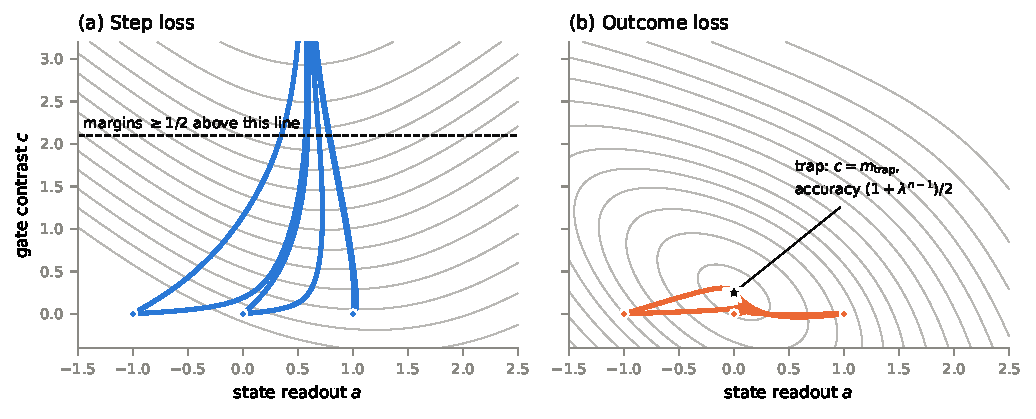
\includegraphics[width=\linewidth]{figures/two_path_phase.pdf}
\caption{\textbf{The same seeds, two losses.} Gradient flow of the two-path family (curves; dots are starting points),
shown in the plane of the state readout $a$ and the gate contrast $g\tanh(qk)$, over level sets of the loss (gray).
(a)~Under the step loss the contrast grows without bound and the margins become positive.
(b)~Under the outcome loss every trajectory converges to the one-letter trap (star). Here $n=4$, so that the
trap is visible; for larger $n$ it moves towards the origin.}
\label{fig:two-path-phase}
\end{figure}

The seeds of \cref{thm:matched} live in the reduced family, not the full Transformer, and are not at small scale:
the gate starts at order one while the averaging path starts small. $\mathcal U_n$ contains, for example, the seed $q_0=k_0=1$ with two active ReLUs of size about
$p/\sqrt{n\log(1/p)}$ and all state weights $d_i=0$, together with every small enough perturbation of it
(\cref{lem:seed-set}); $n_0(1/4)=32$. The conditions ask that every ReLU be on or off over all inputs, that
the averaging path start small compared with the gate, and that the state weights be small compared with
the ReLU margins; the exact form is in \cref{app:matched-proof}.

\emph{Sketch of proof.} \emph{Outcome half.} At zero readout the loss is $\log2$, only
$O(\lambda^{2(n-1)})$ above the trap. Gradient flow turns a small loss gap into a short path, so the flow cannot
leave the region where each ReLU keeps its sign. There the loss is a strictly convex function of four
effective coefficients, and its only minimizer is the trap (\cref{app:random-trap-certificate}).
\emph{Step half.} In the same region the step logit is $AS+BSC+Du+E$, where $B=g\tanh(qk)$ is the gate contrast.
(a)~\emph{The gate grows:} $\dot B\ge\tanh^2(q_0k_0)$ times the current error rate.
(b)~\emph{The state readout is bounded:} $a$ stays in $[0,\log\frac{1-p}p]$ up to small corrections.
(c)~\emph{The averaging path stays small:} it is driven only through the state weights,
\[
 \dot v=\dot a\,d-Gv,\qquad \dot d=\dot a\,v,\qquad G\succeq0,
\]
so $v$ and $d$ grow by at most a factor $O(1/p)$, and the averaging path never competes with the gate.
(d)~\emph{Margins persist:} once the loss is below the smallest cell probability, no margin can turn
negative again (\cref{app:matched-proof}).

The outcome executor is in the family at zero loss, and the same gate path that outcome training leaves
weak is driven to a margin by step training. The trap is therefore caused by the outcome loss, not by
missing capacity: with matched initialization, architecture and expressivity, only the supervision format
differs. This is the controlled counterpart of \cref{thm:outcome-end,thm:routing}.

% ===================================================================
\suppressfloats[t]
\section{Experiments}
\label{sec:experiments}
\label{sec:validation}

We test each theorem with binary counting at $p=1/4$ ($\lambda=1/2$); protocols are in \cref{app:experiments}.

\begin{figure}[t]
\centering
\resizebox{\linewidth}{!}{%% Experiments figure: (a) from overview.tex, (b,c) from theory_measurement.tex (same data sources).
\definecolor{stepc}{HTML}{0072B2}\definecolor{outc}{HTML}{D55E00}\definecolor{theoc}{HTML}{009E73}
\definecolor{mutedc}{HTML}{6E6E6E}\definecolor{errc}{HTML}{EDB79C}
\begin{tikzpicture}
\pgfplotsset{every axis/.style={width=0.4\linewidth, height=4.9cm, axis line style={black!80}, tick style={black!80},
  tick label style={font=\footnotesize}, label style={font=\small}, title style={font=\small, at={(0,1)}, anchor=south west, xshift=-2pt},
  axis x line*=bottom, axis y line*=left}, every axis plot/.append style={line width=1pt}}
\begin{axis}[name=pa, title={\textbf{(a)} Training, $n=16$}, xlabel={Updates (thousands)}, ylabel={Exact accuracy (\%)},
  xmin=0, xmax=8, ymin=0, ymax=112, xtick={0,4,8}, ytick={0,50,100}, axis x line*=bottom, axis y line*=left, clip=false]
  \addplot[draw=none, fill=stepc, fill opacity=0.18, forget plot] coordinates {(1,0.55) (2,0.73) (3,0.82) (4,1.25) (5,9.77) (6,29.75) (7,49.33) (8,98.40) (8,100.00) (7,100.00) (6,100.00) (5,92.03) (4,1.90) (3,1.40) (2,1.35) (1,1.35)};
  \addplot[draw=none, fill=outc, fill opacity=0.18, forget plot] coordinates {(1,49.52) (2,49.73) (3,49.05) (4,48.92) (5,49.35) (6,49.92) (7,48.97) (8,49.15) (8,50.70) (7,50.70) (6,51.20) (5,51.08) (4,50.60) (3,50.70) (2,51.08) (1,51.08)};
  \addplot[theoc, dashed, line width=0.9pt, domain=0:8, samples=2] {100};
  \addplot[mutedc, densely dashed, line width=0.8pt, domain=0:8, samples=2] {50};
  \addplot[stepc, mark=square*, mark size=1.8pt] coordinates {(1,1.00) (2,1.05) (3,1.30) (4,1.45) (5,21.65) (6,73.40) (7,95.40) (8,100.00)};
  \addplot[outc, mark=*, mark size=1.9pt] coordinates {(1,50.40) (2,50.60) (3,50.40) (4,49.85) (5,50.25) (6,50.60) (7,50.25) (8,50.40)};
  \node[anchor=south west, font=\footnotesize, text=theoc, inner sep=1pt] at (axis cs:0.15,101.5) {Exact executor};
  \node[anchor=west, font=\small\bfseries, text=stepc] at (axis cs:0.2,86) {Step};
  \node[anchor=west, font=\scriptsize, text=stepc] at (axis cs:0.2,76) {8/10 seeds solve};
  \node[anchor=south west, font=\small\bfseries, text=outc, inner sep=1pt] at (axis cs:0.15,54) {Outcome};
  \node[anchor=north west, font=\scriptsize, text=mutedc, inner sep=1pt] at (axis cs:0.15,46) {Chance};
\end{axis}
\begin{semilogyaxis}[name=pb, at={(pa.east)}, anchor=west, xshift=1.6cm, title={\textbf{(b)} Plateau duration}, xlabel={Horizon $n$}, ylabel={Displacement time $\tau(0.1)$},
  xmin=3.6, xmax=14.4, xtick={4,8,14}, ymin=3, ymax=1e8, ytick={1e1,1e3,1e5,1e7}, ymajorgrids, major grid style={black!12}]
  \addplot[draw=none, fill=outc, fill opacity=0.18, forget plot] coordinates {(4,10638.7) (6,53401.7) (8,257804) (10,1.17632e+06) (12,5.46642e+06) (14,2.47378e+07) (14,3.29507e+07) (12,6.99489e+06) (10,1.54461e+06) (8,332934) (6,68528) (4,13708.5)};
  \addplot[draw=none, fill=stepc, fill opacity=0.18, forget plot] coordinates {(4,4.2576) (6,4.25798) (8,4.25824) (10,4.25841) (12,4.25855) (14,4.25866) (14,4.94345) (12,4.94354) (10,4.94365) (8,4.9438) (6,4.94399) (4,4.9443)};
  \addplot[outc, mark=*, mark size=1.8pt] coordinates {(4,12013.4) (6,60575.1) (8,290310) (10,1.30468e+06) (12,6.1887e+06) (14,2.74812e+07)};
  \addplot[stepc, mark=square*, mark size=1.7pt] coordinates {(4,4.33272) (6,4.3327) (8,4.33268) (10,4.33266) (12,4.33266) (14,4.33265)};
  \addplot[theoc, dashed, line width=0.9pt] coordinates {(4,12013.4) (6,48053.5) (8,192214) (10,768856) (12,3.07542e+06) (14,1.23017e+07)};
  \node[anchor=west, font=\footnotesize, text=outc] at (axis cs:4,4e6) {Outcome};
  \node[anchor=north east, font=\footnotesize, text=theoc] at (axis cs:14,1.538e+06) {$\mixrate^{-n}$};
  \node[anchor=south, font=\footnotesize, text=stepc] at (axis cs:10,13) {Step};
\end{semilogyaxis}
\begin{semilogxaxis}[name=pc, at={(pb.east)}, anchor=west, xshift=1.75cm, title={\textbf{(c)} Outcome accuracy follows $\mixrate^n$},
  xlabel={Remaining bias $\mixrate^n$}, ylabel={Outcome accuracy (\%)}, xmin=1e-5, xmax=0.8, xtick={1e-5,1e-3,1e-1},
  ymin=0, ymax=103, ytick={0,50,100}, ymajorgrids, major grid style={black!12}]
  \addplot[mutedc, densely dashed, line width=0.8pt, domain=1e-5:0.8, samples=2] {50};
  \addplot[theoc, dashed, line width=1pt, domain=1e-5:0.7, samples=120] {50*(1+x)};
  \addplot[only marks, outc, mark=*, mark size=1.6pt, error bars/.cd, y dir=both, y explicit, error bar style={errc, line width=0.8pt},
    error mark=none] coordinates {(0.015625,49.6) += (0,0.1) -= (0,0.1) (0.0877915,57.33) += (0,2.467) -= (0,1.633) (0.262144,70.33) += (0,5.667) -= (0,6.233) (0.531441,79.03) += (0,2.167) -= (0,1.933) (0.00390625,51.17) += (0,3.833) -= (0,2.367) (0.0390184,51.27) += (0,1.833) -= (0,2.167) (0.167772,61.73) += (0,3.967) -= (0,3.233) (0.430467,70.93) += (0,0.6667) -= (0,0.5333) (0.000976562,50.07) += (0,0.3333) -= (0,0.5667) (0.0173415,50.57) += (0,0.4333) -= (0,0.8667) (0.107374,55.37) += (0,1.233) -= (0,0.9667) (0.348678,71.13) += (0,2.667) -= (0,2.233) (0.000244141,50.37) += (0,0.5333) -= (0,0.9667) (0.00770735,51.93) += (0,1.467) -= (0,1.433) (0.0687195,51.53) += (0,4.367) -= (0,2.833) (0.28243,64.4) += (0,1.7) -= (0,1.7) (1.52588e-05,50.4) += (0,1.2) -= (0,1.1) (0.00152244,50.2) += (0,1) -= (0,1.3) (0.0281475,50.47) += (0,2.233) -= (0,2.967) (0.185302,57.23) += (0,1.867) -= (0,2.733)};
  \node[anchor=north west, font=\footnotesize] at (rel axis cs:0.03,0.98) {Spearman $\rho=0.91$};
  \node[anchor=north west, font=\footnotesize, text=theoc] at (rel axis cs:0.03,0.8) {State-only prior};
  \node[anchor=north west, font=\scriptsize, text=mutedc] at (rel axis cs:0.03,0.46) {Chance};
\end{semilogxaxis}
\end{tikzpicture}
}
\caption{\textbf{Outcome training stalls on an exponential plateau; step training does not.}
(a)~Full Transformer, $n=16$, zero readout, AdamW: median exact continuation accuracy and interquartile band over ten
paired seeds. Both formats admit an exact executor (\cref{prop:represent}).
(b)~Small initialization ($\varepsilon=0.002$): time for training to move a fixed distance from the seed, median and
interquartile band over three draws; the dashed guide is $\lambda^{-n}$ (\cref{thm:outcome-end}).
(c)~Outcome accuracy after $8$k updates in $20$ horizon--alphabet cells (means and seed ranges) against $\lambda^n$;
the dashed curve is the accuracy $\frac{1+\lambda^n}2$ of the state-only prior.}
\label{fig:experiments}
\end{figure}

\paragraph{Does outcome training stall for time $\lambda^{-n}$? (\cref{thm:outcome-end})} With $n=16$, step training solves
$8$ of $10$ seeds while outcome training stays at chance (\cref{fig:experiments}a). In the small-initialization
regime the time to leave the seed grows from $10^4$ at $n=4$ to $3\times10^7$ at $n=14$, at least as fast as
$\lambda^{-n}$, while the step exit time stays at $4.3$ for every $n$ (\cref{fig:experiments}b). No ReLU changes sign
along these runs. Across horizons and alphabets, what outcome training learns is the state-only prior
$\frac{1+\lambda^n}2$ (Spearman $\rho=0.91$) and essentially nothing beyond it (median excess $0.2$ points,
\cref{fig:experiments}c).

\paragraph{Can step training learn the routing jointly? (\cref{thm:routing})} Training query--key maps, relative biases and readout
together from a random initialization solves $16$ of $17$ step runs, and the last reaches $99.95\%$. Matched outcome
runs solve none within $300$k updates (\cref{tab:reach}). Step solve times grow from $44$k updates at $n=6$ to
$237$k at $n=16$, far below the $1{,}024$-fold growth of $\lambda^{-n}$.

\begin{table}[t]
\caption{\textbf{Step training learns the routing; outcome training under the same protocol does not.}
Scores, relative bias and readout are trained by full-batch gradient descent from $\varepsilon=0.3$, with the same seeds for both
formats. Solved: every held-out prediction correct.}
\label{tab:reach}
\centering\small
\begin{tabular}{@{}rcccc@{}}
\toprule
 & \multicolumn{2}{c}{Step} & \multicolumn{2}{c}{Outcome (300k updates)}\\
\cmidrule(lr){2-3}\cmidrule(l){4-5}
$n$ & Solved & Updates to solve, median (range) & Solved & Answer accuracy (\%)\\
\midrule
6  & 5/5 & 44k (41--78k)   & 0/5 & 50--94\\
8  & 5/5 & 61k (46--99k)   & 0/5 & 50--55\\
12 & 4/5 & 77k (42--103k)  & 0/5 & 50\\
16 & 2/2 & 237k (208--266k) & 0/2 & 50--51\\
\bottomrule
\end{tabular}
\end{table}

\paragraph{Does the same family split as \cref{thm:matched} predicts?} We run population gradient descent (step sizes $1$, $\tfrac12$ and $\tfrac14$, giving the same results) in
the two-path family from $12$ seeds that satisfy every condition of $\mathcal U_n$, checked numerically, at
$n\in\{36,40,48,64\}$: perturbations of the explicit seed with nonzero state weights on all units. Every transition
reaches margin $1/2$ by flow time $5$, far inside the bound of \cref{thm:matched} ($T\approx265$ for these seeds, an upper bound); outcome training ends after flow time $2\times10^4$ at
exactly the one-letter accuracy $(1+\lambda^{n-1})/2$, with no ReLU changing sign. Away from these seeds
(Appendix, \cref{fig:two-path-sweep}), outcome training never escapes at $n=17$, and escapes at $n=6,8$ only when
ReLU kinks start inside the input range.

\paragraph{Is the advantage just more labels?} \input{sections/label_budget_result}

% ===================================================================
\section{Related work and limitations}
\label{sec:related}
\label{sec:conclusion}

\paragraph{Related work.} Intermediate supervision has been studied through decomposition, locality,
expressivity and sample complexity
\citep{wies2023subtask,prystawski2023think,abbe2024globality,feng2023towards,merrill2024expressive,malach2023autoregressive,hanneke2026samplecomplexityautoregressivereasoning,wen2024sparse};
we fix the target and architecture and follow the gradient instead. Our credit bound is in the spirit of
failures of gradient learning for orthogonal targets \citep{shalevshwartz2017failures} and of
initialization-dependent parity learning \citep{abbe2025parities}, and is related to staircase and low-degree
analyses \citep{abbe2021staircase,abbe2023sgd,panigrahi2025progressive}; the new ingredient is a Transformer score
expansion that bounds how many letters each term reads. \citet{makkuva2025attention,makkuva2024local}
characterize good and bad minima of single-layer Transformers on Markov chains. \Citet{kim2024parity} are
discussed in \cref{sec:intro}. Counting is a cyclic automaton whose shallow shortcuts exist
\citep{liu2023automata}; we show that existence does not mean training finds them.

\paragraph{Limitations.} The negative results for the full Transformer hold near small initialization;
outside it we have experiments, and one counterexample: for counting modulo $3$ at $n=8$, where
$\lambda^{-8}\approx27$ is modest, two of three AdamW outcome runs solve the task (\cref{app:spectrum}).
The matched theorem supplies routing and averaging and needs $n\ge n_0(p)$; its seed conditions are sufficient,
not necessary. Learning routing and unrestricted features jointly from random weights remains open.
